\documentclass{article}
\usepackage[submission]{colm2026_conference}

\usepackage{microtype}
\usepackage[colorlinks=false,pdfborder={0 0 0}]{hyperref}
\input{math_commands}
\usepackage{url}
\usepackage{booktabs}
\usepackage{algorithm}
\usepackage{algorithmic}
\usepackage{tikz}
\usetikzlibrary{shapes,arrows.meta,positioning,fit,calc,decorations.pathreplacing}
\usepackage{pgfplots}
\pgfplotsset{compat=1.18}
\usepackage{listings}
\usepackage{multirow}
\usepackage{amsmath}
\usepackage{amssymb}
\usepackage{xcolor}
\usepackage{enumitem}
\usepackage{subcaption}
\usepackage{float}
\usepackage{tabularx}
\renewcommand{\arraystretch}{1.15}   % more row height
\setlength{\tabcolsep}{4pt}          % less column padding

% Custom colors from main_1.tex
\definecolor{agentblue}{RGB}{66,133,244}
\definecolor{routergreen}{RGB}{52,168,83}
\definecolor{dilutionred}{RGB}{234,67,53}
\definecolor{codebg}{RGB}{245,245,245}
\definecolor{hybridgold}{RGB}{204,153,0}

% Custom commands from main_1.tex
\newcommand{\systemname}{\textsc{MASDR-RAG}}
\newcommand{\hybridname}{\textsc{Hybrid-Routed}}
\newcommand{\todo}[1]{\textcolor{red}{\textbf{[TODO: #1]}}}
\newcommand{\numDocs}{1{,}128}
\newcommand{\numChunks}{88{,}907}
\newcommand{\numQueries}{200}
\newcommand{\sig}{$^{**}$}
\newcommand{\sigsingle}{$^{*}$}

% Listings setup
\lstset{
  basicstyle=\ttfamily\small,
  backgroundcolor=\color{codebg},
  breaklines=true,
  frame=single,
  framerule=0.5pt,
  columns=fullflexible
}

\title{When More Documents Hurt RAG: Mitigating Vector Search Dilution with Domain-Scoped Multi-Agent Retrieval}

\author{Anonymous Authors \\
Affiliation \\
Address \\
\texttt{email}
}

\newcommand{\fix}{\marginpar{FIX}}
\newcommand{\new}{\marginpar{NEW}}
\begin{document}
\maketitle

% ============================================================
% ABSTRACT
% ============================================================
\begin{abstract}
Retrieval-Augmented Generation (RAG) systems degrade when scaled to large document collections. As the number of heterogeneous documents grows, embedding-based similarity becomes less useful as it increasingly retrieves semantically similar but irrelevant chunks. We call this problem \textit{vector search dilution}.
We collect real-world documents from the Wyoming Department of Transportation (WYDOT), consisting of 1,128 documents and \numChunks{} chunks. In a small subset (54 documents), the system achieved 58\% answer accuracy. However, when we evaluated the same system on the entire document collection, the precision decreased to 54\%. This shows that scaling the corpus reduces retrieval quality. We analyze the reasons for this drop and identify two main causes: vocabulary overlap across different document categories and imbalance in chunk distribution. To address this, we propose \systemname{} (Multi-Agent Scoped Domain Retrieval for RAG). Our approach uses domain-scoped retrieval over a Neo4j knowledge graph combined with hybrid query routing. We evaluate our system in five configurations using \numQueries{} AI-curated queries with manual validation. Our results reveal a precision--faithfulness paradox: domain scoping improves retrieval precision (P@10: 0.77 $\rightarrow$ 0.86, $p < 0.05$), but naive multi-agent orchestration reduces answer faithfulness (0.61 $\rightarrow$ 0.35, $p < 0.01$) due to context fragmentation. We show that the \hybridname{} routing resolves this issue. It improves retrieval precision (P@10: 0.83) while maintaining faithfulness (0.62, $p = 0.90$ compared to baseline). The code and data will be made public upon acceptance.

% Code and data will be released upon acceptance.
\end{abstract}

% ============================================================
% 1. INTRODUCTION
% ============================================================
\section{Introduction}
\label{sec:introduction}

Retrieval-Augmented Generation (RAG) has emerged as a dominant approach for incorporating external knowledge into large language model (LLM) outputs ~\citep{lewis2020rag, guu2020realm}. By retrieving relevant passages from a document corpus before generation, RAG systems help mitigate hallucinations ~\citep{shuster2021retrieval, huang2024hallucination}, provide access to private or domain-specific data ~\citep{gao2024ragsurvey}, and avoid the high cost of fine-tuning ~\citep{izacard2023atlas}. The standard RAG pipeline, including document embedding, building a vector index, retrieving the top-$k$ similar chunks, and feeding them to an LLM, works well for small, homogeneous corpora.

There is a gap between laboratory-scale RAG experiments, which typically use curated datasets of tens to hundreds of documents ~\citep{kwiatkowski2019natural, joshi2017triviaqa}, and production deployments that must handle thousands of heterogeneous documents. As organizations digitize their knowledge bases, RAG systems are increasingly tasked with managing document collections spanning multiple domains, formats, and time periods~\citep{barnett2024seven}. This scaling challenge is particularly acute in government and enterprise settings, where document collections can grow by orders of magnitude during deployment ~\citep{wu2025rag4cm}.

In this paper, we identify and study \textit{vector search dilution}, a phenomenon in which embedding-based retrieval loses discriminative power as the corpus scales across heterogeneous categories. Unlike traditional scalability issues in approximate nearest neighbor (ANN) algorithms ~\citep{malkov2020hnsw, johnson2021faiss}, vector search dilution is a semantic problem. When documents from different domains share overlapping vocabulary, embedding models produce similar vectors for semantically related but contextually irrelevant chunks. As a result, top-$k$ retrieval often returns cross-domain noise, reducing the quality of downstream generation.

We grounded our analysis in a real-world case study: a knowledge graph-powered RAG chatbot deployed for heterogeneous transportation documents. When the system scaled from 54 to \numDocs{} documents in 9 domain categories, the response quality decreased from 58\% to 54\%. 
% Queries about construction specifications erroneously returned crash report statistics. Similarly, materials testing queries retrieved irrelevant bridge design documents.
To address this scaling challenge, we propose \systemname{}, a novel architecture that combines hybrid query routing with domain-scoped multi-agent retrieval over a knowledge graph. 
By evaluating this architecture across five configurations, we uncover a key empirical finding: the \textit{precision--faithfulness paradox}. While domain scoping substantially improves retrieval precision, naive multi-agent orchestration can degrade answer faithfulness due to context fragmentation across multiple tool calls. We demonstrate that our hybrid routing mechanism resolves this paradox by reducing unnecessary multi-agent dispatch (\S\ref{sec:paradox}).

% Our contributions are:
% \begin{enumerate}[leftmargin=*,topsep=2pt,itemsep=1pt]
%     \item The first systematic diagnosis and formal characterization of vector search dilution in a production RAG system, with empirical measurements across 8 document categories (\S\ref{sec:dilution}).
%     \item A complete architecture combining hybrid routing, graph-based scoping, and multi-agent orchestration, evaluated across six system configurations (\S\ref{sec:architecture}).
%     \item Identification of the precision--faithfulness paradox, showing that retrieval improvements do not automatically translate to answer quality improvements, with analysis of root causes (\S\ref{sec:paradox}).
%     \item Practical guidelines for when dilution becomes critical, how to determine optimal agent granularity, and techniques for reducing latency and cost while improving reasoning (\S\ref{sec:paradox}).
% \end{enumerate}
Our contributions are:
\begin{enumerate}[leftmargin=*,topsep=2pt,itemsep=1pt]
    \item A systematic characterization of \emph{vector search dilution} in a production RAG system, with empirical analysis across eight document categories (\S\ref{sec:dilution}).
    \item A hybrid RAG architecture that combines routing, graph-based scoping, and multi-agent orchestration, evaluated across five system configurations (\S\ref{sec:architecture}).
    \item An analysis of the precision--faithfulness paradox, showing why retrieval gains do not necessarily improve answer quality, along with practical guidelines for mitigating dilution while reducing latency and cost (\S\ref{sec:paradox}).
\end{enumerate}


% ============================================================
% 2. RELATED WORK
% ============================================================
\section{Related Work}
\label{sec:related_work}

\paragraph{RAG and Dense Retrieval.}
The RAG paradigm ~\citep{lewis2020rag} is built on open-domain QA with retrieval ~\citep{chen2017drqa, karpukhin2020dpr}. The evolution from naive to advanced RAG -- with query transformation, re-ranking, and iterative retrieval -- is well documented \citep{gao2024ragsurvey, zhao2024ragsurvey2}. Recently, the community has identified \textit{agentic RAG} ~\citep{singh2025agenticrag}, where autonomous agents decide when and how to retrieve. Dense retrieval ~\citep{karpukhin2020dpr, xiong2021ance} has largely supplanted sparse methods ~\citep{robertson2009bm25}, although hybrid approaches remain competitive ~\citep{sawarkar2024blended}. Scaling challenges are typically framed in terms of ANN performance: HNSW ~\citep{malkov2020hnsw}, FAISS ~\citep{johnson2021faiss}, and ScaNN ~\citep{guo2020scann} address computational efficiency. We identify a distinct \textit{semantic} scaling problem: even when an ANN returns the true nearest neighbors, those neighbors may be irrelevant due to embedding space contamination. This complements \citet{barnett2024seven} on RAG failures, but provides the first formal characterization.

\paragraph{Query Routing and Multi-Agent Systems.}
Adaptive-RAG routes~\citep{jeong2024adaptiverag} by complexity; RAGRouter~\citep{zhang2025ragrouter} and RouteRAG~\citep{guo2025routerag} train classifiers for strategy selection; Multi-Meta-RAG~\citep{poliakov2024multimetarag} uses metadata filtering. Our routing is distinct: we route by \textit{document domain} rather than by strategy, and we show that a \textit{hybrid} approach (rule-based + LLM) outperforms either approach alone. For multi-agent systems, ReAct ~\citep{yao2023react}, Toolformer ~\citep{schick2023toolformer}, and AutoGen ~\citep{wu2023autogen} provide general frameworks. MA-RAG~\citep{nguyen2025marag} applies multiple agents to RAG. Our agents serve as \textit{domain gatekeepers} — each restricting search to a subset of documents. Critically, we show that multi-agent orchestration introduces \textit{context fragmentation} that degrades faithfulness, a finding not reported in prior work.

\paragraph{Graph-Enhanced and Domain-Partitioned RAG.}
GraphRAG ~\citep{edge2024local} builds entity-relationship graphs; HybridRAG ~\citep{sarmah2024hybridrag} combines KG traversal with vector similarity; KG-RAG ~\citep{sanmartin2024kgrag} increases biomedical QA. We leverage the graph's \textit{organizational metadata} as agent boundaries rather than entity relationships for retrieval. Several systems partition retrieval by domain in engineering settings~\citep {masoudifard2024leveraging}. Our contribution is the \textit{explicit diagnosis} of why partitioning helps (dilution) and when it hurts (the precision--faithfulness paradox).

\paragraph{RAG Evaluation:}
Retreival Augmenented Generation Assessment(RAGAS)~\citep{es2024ragas} measures faithfulness, relevance, and context precision. Standard benchmarks such as Natural Questions~\citep{kwiatkowski2019natural} and MS MARCO ~\citep{nguyen2016msmarco} use homogeneous corpora and do not capture cross-domain dilution effects.

\section{Vector Search Dilution}
\label{sec:dilution}

\subsection{System Context}

The corpus comprises \numDocs{} documents that span construction specifications, design manuals, material testing procedures, crash reports, transportation improvement programs, and administrative reports. These were ingested into a Neo4j knowledge graph with the following hierarchy:
\begin{equation}
\text{Document} \xrightarrow{\text{CONTAINS}} \text{Section} \xrightarrow{\text{CONTAINS}} \text{Chunk}
\end{equation}

The chunks were embedded using Google's Gemini Embedding model (\texttt{gemini-embedding-001}, 768 dimensions) and indexed with an HNSW vector index and a BM25 full-text index. The system uses hybrid search ~\citep{sawarkar2024blended} with Gemini 2.5 Flash for generation. The knowledge graph contains 152,231 nodes and 338,569 relationships.
Traffic \& Crash reports constitute 35\% of chunks despite being 2\% of documents, creating an extreme 54$\times$ chunk density variance across categories (see Appendix~\ref{app:distribution} for the full table).


\subsection{Scaling and Degradation}

The system was implemented in two phases: V1 (54 documents, 1,600 chunks, primarily standard specifications) achieved 58\% accuracy, while V2 scaled to \numDocs{} documents and \numChunks{} chunks across 8 categories, dropping overall accuracy to 54\%. This 20-fold increase in document count yielded a 55-fold increase in chunks due to variable chunk densities across document types. Although the absolute accuracy drop was a modest 4 points, it masks severe category-specific degradation, with the Standard Specs query accuracy collapsing from 75\% to below 40\%.

\subsection{Root Cause Analysis}

\paragraph{Vocabulary Overlap:} Transportation documents share extensive domain vocabulary across categories. 
General-purpose embedding models ~\citep{reimers2019sentencebert, wang2024e5mistral} cannot disambiguate these domain-specific usages because they lack a training signal for organizational document boundaries.

For ``What is the surface grinding threshold for concrete pavement?'' targeting Standard Specs Section 401:
\begin{itemize}[leftmargin=*,topsep=2pt,itemsep=1pt]
    \item 30,922 crash chunks containing ``surface condition'' produce high cosine similarity
    \item Bridge ``surface preparation'' chunks add additional noise
    \item Target specs chunks ($\sim$2,500) are numerically overwhelmed
\end{itemize}

\paragraph{Chunk Distribution Imbalance:} Document types vary dramatically in chunk density (Appendix~\ref{app:distribution}). Crash report PDFs contain dense statistical tables that recursive text splitters ~\citep{langchain2024recursive} fragment into thousands of small chunks. A single 2021 crash report (133 pages) generated 14,891 chunks, while the entire Standard Specifications produced only $\sim$2,500. This creates a \textit{de facto} oversampling of high-density categories in the embedding space.

\subsection{Formal Definition}

Let $\mathcal{C} = \{c_1, \ldots, c_N\}$ be $N$ chunks partitioned into $K$ categories $\mathcal{C}_1, \ldots, \mathcal{C}_K$. Let $e: \mathcal{C} \rightarrow \mathbb{R}^d$ be an embedding function and $q$ a query targeting category $k^*$. The top-$m$ retrieval set is:
\begin{equation}
R_m(q) = \underset{S \subseteq \mathcal{C}, |S|=m}{\arg\max} \sum_{c \in S} \text{sim}(e(q), e(c))
\end{equation}

\textit{Vector search dilution} occurs when global retrieval precision is substantially lower than scoped precision:
\begin{equation}
\text{P}_{\text{global}} = \frac{|R_m(q) \cap \mathcal{C}_{k^*}|}{m} \ll \frac{|R_m^{k^*}(q) \cap \mathcal{C}_{k^*}|}{m} = \text{P}_{\text{scoped}}
\end{equation}

The \textit{dilution factor}:
\begin{equation}
\delta(q, k^*) = 1 - \frac{\text{P}_{\text{global}}(q)}{\text{P}_{\text{scoped}}(q)}
\label{eq:dilution}
\end{equation}

where $\delta = 0$ indicates no dilution and $\delta \rightarrow 1$ indicates severe dilution. The dilution is related to but distinct from the drift of topics~\citep{allan2002tdt}: it is caused by the corpus's static composition rather than by the evolution of dynamic topics.

\subsection{Empirical Dilution Measurements}

Table~\ref{tab:dilution} presents empirical dilution measurements across 8 domain categories using the full \numQueries{}-query evaluation ($n = 4$--$23$ queries per category). Categories with smaller chunk populations suffer the most severe dilution: the Design Manual ($\delta = 0.53$, 1,405 chunks) loses 53\% of its retrieval precision when searched globally vs.\ scoped, while the Construction Manual ($\delta = 0.10$, 6,641 chunks) has a sufficiently distinct vocabulary to largely resist dilution. The Spearman rank correlation between $\log(\text{chunk count})$ and mean $\delta$ across 8 categories is $\rho = -0.60$ ($p = 0.12$), suggesting --but not definitively establishing---an inverse relationship between corpus size and dilution severity.

\begin{table}[H]
\centering
\footnotesize
\begin{tabular}{l r r r r}
\toprule
\textbf{Category} & \textbf{Chunks} & \textbf{$\delta$ (mean)} & \textbf{$\delta$ (range)} & \textbf{$n$} \\
\midrule
Design Manual       & 1,405  & 0.53 & 0.00--1.00 & 12 \\
Standard Specs      & 2,519  & 0.43 & 0.00--1.00 & 23 \\
Materials Testing   & 2,180  & 0.22 & 0.00--0.50 & 20 \\
Bridge Program      & 5,399  & 0.21 & 0.00--0.70 & 12 \\
STIP                & 13,634 & 0.17 & 0.00--0.70 & 9 \\
Traffic \& Crashes  & 30,922 & 0.16 & 0.00--0.60 & 7 \\
Annual Reports      & 2,341  & 0.12 & 0.00--0.30 & 4 \\
Construction Manual & 6,641  & 0.10 & 0.00--0.80 & 21 \\
\bottomrule
\end{tabular}
\caption{Dilution factor $\delta$ by category with per-query ranges. Categories with fewer chunks tend to suffer higher dilution (Spearman $\rho=-0.60$, $p=0.12$, $n=8$ categories). The high variance within categories (e.g., Standard Specs: 0.00--1.00) reflects query-level sensitivity to vocabulary overlap.}
\label{tab:dilution}
\end{table}

% Figure removed to save space — data presented in Table~\ref{tab:dilution}.



% %============================================================
% 4. ARCHITECTURE
% ============================================================
\section{Architecture: \systemname{}}
\label{sec:architecture}

Our architecture has three major components:

\begin{enumerate}[leftmargin=*,topsep=2pt,itemsep=1pt]
    \item \textbf{Domain-scoped retrieval via knowledge graph metadata}: Each domain agent restricts search to document subsets defined by Neo4j graph metadata, reducing the effective search space by 85--98\% (\S\ref{sec:scoped_search}).
    \item \textbf{Hybrid query routing}: A combination of rule-based pattern matching (47\% accuracy, 50\% coverage) and LLM zero-shot classification (57\% accuracy, 100\% coverage), with the rule-based router taking precedence when confident (\S\ref{sec:routing}).
    \item \textbf{Multi-agent orchestration with tool calling}: A Gemini-based orchestrator uses function calling to dispatch queries to specialized agents, enabling multi-hop reasoning and cross-domain comparison (\S\ref{sec:orchestrator}).
\end{enumerate}


\newcommand{\numAgents}{9}

\begin{figure}[H]
\centering
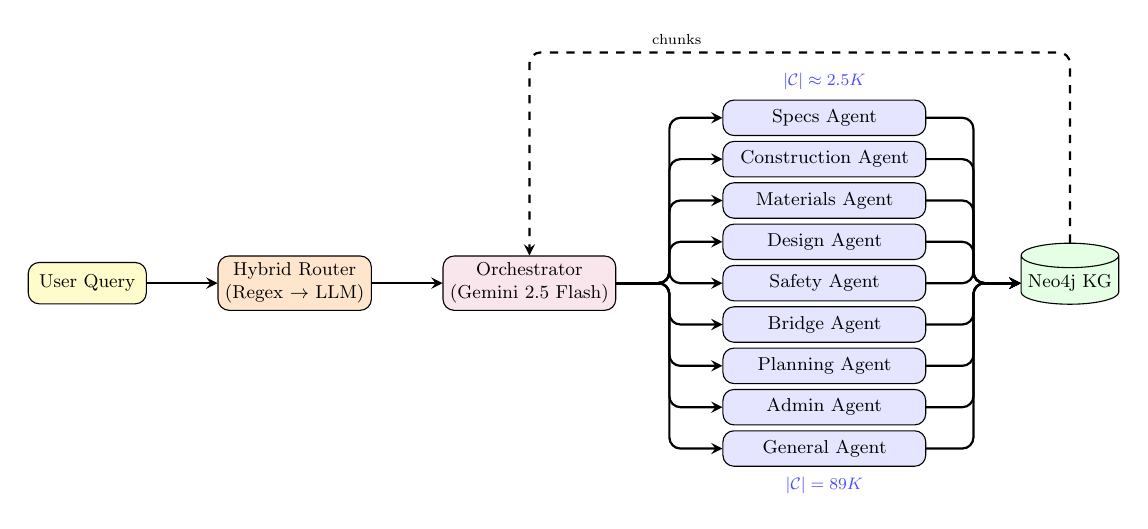
\begin{tikzpicture}[scale=0.75, every node/.style={transform shape},
    node distance=0.6cm and 1.2cm,
    box/.style={rectangle, draw, rounded corners, minimum width=2cm, minimum height=0.7cm, align=center, font=\small},
    agent/.style={rectangle, draw, fill=blue!10, rounded corners, text width=3.2cm, minimum height=0.6cm, align=center, font=\small},
    db/.style={cylinder, draw, fill=green!10, shape border rotate=90, minimum width=1.0cm, minimum height=0.7cm, font=\small, aspect=0.25},
    arrow/.style={->, >=stealth, thick},
]
    \node[box, fill=yellow!20] (query) {User Query};
    \node[box, fill=orange!20, right=1.2cm of query] (router) {Hybrid Router\\(Regex $\rightarrow$ LLM)};
    \node[box, fill=purple!10, right=1.2cm of router] (orch) {Orchestrator\\(Gemini 2.5 Flash)};
    \node[agent, right=1.8cm of orch, yshift=2.8cm] (specs) {Specs Agent};
    \node[agent, right=1.8cm of orch, yshift=2.1cm] (const) {Construction Agent};
    \node[agent, right=1.8cm of orch, yshift=1.4cm] (mats) {Materials Agent};
    \node[agent, right=1.8cm of orch, yshift=0.7cm] (design) {Design Agent};
    \node[agent, right=1.8cm of orch, yshift=0.0cm] (safety) {Safety Agent};
    \node[agent, right=1.8cm of orch, yshift=-0.7cm] (bridge) {Bridge Agent};
    \node[agent, right=1.8cm of orch, yshift=-1.4cm] (plan) {Planning Agent};
    \node[agent, right=1.8cm of orch, yshift=-2.1cm] (admin) {Admin Agent};
    \node[agent, right=1.8cm of orch, yshift=-2.8cm] (general) {General Agent};
    \node[db, right=1.6cm of safety] (neo4j) {Neo4j KG};

    \draw[arrow] (query) -- (router);
    \draw[arrow] (router) -- (orch);
    \coordinate (orch_bus) at ($ (orch.east) + (0.9cm, 0) $);
    \draw[arrow, rounded corners] (orch.east) -- (orch_bus) |- (specs.west);
    \draw[arrow, rounded corners] (orch.east) -- (orch_bus) |- (const.west);
    \draw[arrow, rounded corners] (orch.east) -- (orch_bus) |- (mats.west);
    \draw[arrow, rounded corners] (orch.east) -- (orch_bus) |- (design.west);
    \draw[arrow, rounded corners] (orch.east) -- (orch_bus) |- (safety.west);
    \draw[arrow, rounded corners] (orch.east) -- (orch_bus) |- (bridge.west);
    \draw[arrow, rounded corners] (orch.east) -- (orch_bus) |- (plan.west);
    \draw[arrow, rounded corners] (orch.east) -- (orch_bus) |- (admin.west);
    \draw[arrow, rounded corners] (orch.east) -- (orch_bus) |- (general.west);
    
    \draw[arrow, rounded corners] (specs.east) -- ($ (specs.east) + (0.8cm, 0) $) |- (neo4j.west);
    \draw[arrow, rounded corners] (const.east) -- ($ (const.east) + (0.8cm, 0) $) |- (neo4j.west);
    \draw[arrow, rounded corners] (mats.east) -- ($ (mats.east) + (0.8cm, 0) $) |- (neo4j.west);
    \draw[arrow, rounded corners] (design.east) -- ($ (design.east) + (0.8cm, 0) $) |- (neo4j.west);
    \draw[arrow, rounded corners] (safety.east) -- ($ (safety.east) + (0.8cm, 0) $) |- (neo4j.west);
    \draw[arrow, rounded corners] (bridge.east) -- ($ (bridge.east) + (0.8cm, 0) $) |- (neo4j.west);
    \draw[arrow, rounded corners] (plan.east) -- ($ (plan.east) + (0.8cm, 0) $) |- (neo4j.west);
    \draw[arrow, rounded corners] (admin.east) -- ($ (admin.east) + (0.8cm, 0) $) |- (neo4j.west);
    \draw[arrow, rounded corners] (general.east) -- ($ (general.east) + (0.8cm, 0) $) |- (neo4j.west);
    \draw[arrow, dashed, rounded corners] (neo4j.north) |- ([yshift=0.8cm]specs.north) -| node[pos=0.25, above, font=\scriptsize] {chunks} (orch.north);

    \node[font=\footnotesize\itshape, text=blue!70, above=0.05cm of specs] {$|\mathcal{C}| \approx 2.5K$};
    \node[font=\footnotesize\itshape, text=blue!70, below=0.05cm of general] {$|\mathcal{C}| = 89K$};
\end{tikzpicture}
\caption{\systemname{} architecture. The hybrid router first attempts regex matching; if that fails, an LLM classifies the query. The orchestrator dispatches to domain agents via function calling, each searching a scoped subset of the knowledge graph. Dashed arrow: chunks returned for answer synthesis.}
\label{fig:architecture}
\end{figure}

\subsection{Hybrid Query Routing}
\label{sec:routing}

We employ a two-stage routing strategy that combines the precision of rule-based matching with the coverage of LLM classification:

\paragraph{Stage 1: Regex Router:} Pattern matching on explicit category markers (e.g., ``Section 414'' $\rightarrow$ STANDARD\_SPECS, ``construction manual'' $\rightarrow$ CONSTRUCTION\_MANUAL). Coverage: 50\% of queries. Accuracy on covered queries: 47\%.

\paragraph{Stage 2: LLM Router:} For queries not matched by regex, Gemini 2.5 Flash classifies into one of 10 categories (Appendix~\ref{app:categories}) using zero-shot prompting (Appendix~\ref{app:routing_prompt}). The prompt extracts are as follows: \texttt{CATEGORY}, \texttt{YEAR}, and \texttt{SERIES}. Coverage: 100\%. Accuracy: 57\%.

% Category taxonomy table in Appendix~\ref{app:categories}.

The hybrid approach addresses a key limitation of LLM-only routing: while the LLM achieves 100\% coverage, its 57\% accuracy means nearly half of queries may be misrouted. Regex routing, though limited in coverage, provides deterministic correctness for queries with explicit markers, reducing the number of queries dependent on LLM classification.

\subsection{Domain-Scoped Retrieval}
\label{sec:scoped_search}

For agent $a$ with document filter $F_a$, the scoped retrieval is:
\begin{equation}
R_m^a(q) = \underset{S \subseteq \mathcal{C}_{F_a}, |S|=m}{\arg\max} \sum_{c \in S} \text{sim}(e(q), e(c))
\end{equation}
where $\mathcal{C}_{F_a} = \{c \in \mathcal{C} : \text{doc}(c).\text{series} \in F_a\}$. Filters are Cypher WHERE clauses on \texttt{document\_series} properties in the Neo4j knowledge graph (Appendix~\ref{app:filters}).

Within each scope, we perform hybrid search ~\citep{sawarkar2024blended}: (1) vector top-$k$ via HNSW cosine similarity, (2) fulltext top-$k$ via BM25, (3) merge with priority deduplication (vector results preferred on collision).

\begin{table}[t]
\centering
\footnotesize
\begin{tabular}{l r r r}
\toprule
\textbf{Agent} & \textbf{Scope Size} & \textbf{Docs} & \textbf{Reduction} \\
\midrule
Specs         & 3,140  & 22    & 96.5\% \\
Construction  & 6,641  & 21    & 92.5\% \\
Materials     & 2,184  & 7     & 97.5\% \\
Design        & 1,366  & 21    & 98.5\% \\
Safety        & 30,922 & 22    & 65.2\% \\
Bridge        & 8,076  & 45    & 90.9\% \\
Planning      & 13,607 & 58    & 84.7\% \\
Admin         & 2,439  & 47    & 97.3\% \\
General       & 88,907 & 1,128 & 0\% \\
\midrule
\textbf{Wtd.\ Avg.} & -- & -- & \textbf{90.4\%} \\
\bottomrule
\end{tabular}
\caption{Search space reduction per agent. Most agents search $<$5\% of the total corpus. Agent scope sizes are derived from Neo4j \texttt{document\_series} metadata filtering.}
\label{tab:search_space}
\end{table}

\subsection{Multi-Agent Orchestration}
\label{sec:orchestrator}

The orchestrator uses Gemini 2.5 Flash function calling with 11 tool declarations: 9 domain searches + \texttt{compare\_versions} + \texttt{get\_section}.

\begin{algorithm}[H]
\small
\caption{\systemname{} Orchestration}
\label{alg:orchestrator}
\begin{algorithmic}[1]
\REQUIRE Query $q$, history $H$, tools $T$, max iters $I{=}5$
\ENSURE Answer $a$, sources $S$
\STATE $msgs \leftarrow [\text{sys\_prompt}, H, q]$; $S \leftarrow \emptyset$
\FOR{$i = 1$ to $I$}
    \STATE $resp \leftarrow \text{Gemini}(msgs, T)$
    \IF{$resp$ has tool calls}
        \FORALL{$(t, args)$ in $resp$}
            \STATE $chunks \leftarrow \text{REGISTRY}[t].\text{search}(args)$
            \STATE $S \leftarrow S \cup \text{sources}(chunks)$
        \ENDFOR
        \STATE Append results to $msgs$
    \ELSE
        \RETURN $resp.\text{text}, S$
    \ENDIF
\ENDFOR
\RETURN timeout, $S$
\end{algorithmic}
\end{algorithm}

This enables: \textbf{multi-hop reasoning} (search domain A, analyze, search domain B), \textbf{cross-domain comparison} (compare\_versions across years), \textbf{parallel retrieval} (concurrent tool calls), and \textbf{self-correction} (additional searches when results are insufficient). However, as we show in \S\ref{sec:paradox}, this flexibility comes at a cost in achieving faithfulness.


% ============================================================
% 5. IMPLEMENTATION
% ============================================================
\section{Evaluation}
\label{sec:evaluation}

\subsection{Setup}


We constructed a test suite of \numQueries{} queries generated with Gemini 2.5 Flash from the document corpus, which we subsequently validated and corrected through manual review. The queries span five types: single-domain (113), cross-domain (31), version comparison (27), section lookup (22), and ambiguous or general queries (7). For each query, the ground truth was manually verified to include the correct target category, the relevant sections of the documents, and a reference answer. The correctness of the answers was evaluated using the judgment of binary experts by comparing the output of the system with the reference answers with a semantic similarity threshold of $\geq 0.8$.

To evaluate system performance, we report multiple metrics that capture both retrieval and generation quality: Precision@$k$ and Recall@$k$ ($k \in \{5, 10\}$) for retrieval effectiveness; binary correctness for answer accuracy; faithfulness and relevance using RAGAS for generation quality; routing accuracy to assess the router; and end-to-end latency. All reported metrics include 95\% bootstrap confidence intervals computed over 10,000 resamples. Pairwise system comparisons were conducted using permutation tests with $n = 10{,}000$ samples at a significance level of $\alpha = 0.05$.

We evaluate five system configurations: (1) a monolithic baseline using a standard hybrid search over the full corpus; (2) Mono+RRF, which replaces priority deduplication with reciprocal rank fusion ~\citep{cormack2009rrf}; (3) LLM+Scoped, which employs zero-shot LLM-based routing with domain-scoped search; (4) \systemname{}, which uses full multi-agent orchestration with LLM routing; and (5) \hybridname{}, which combines regex-based pre-routing with LLM routing and single-agent scoped search.


\subsection{Routing Evaluation}
\label{sec:routing_eval}

\begin{table}[H]
\centering
\footnotesize
\begin{tabular}{l c c c}
\toprule
\textbf{Router} & \textbf{Coverage} & \textbf{Accuracy} & \textbf{Latency} \\
\midrule
Regex & 50\% & 47\% & $<\!$1\,ms \\
LLM (Gemini Flash) & 100\% & 57\% & 200--400\,ms \\
Hybrid (Regex $\rightarrow$ LLM) & 100\% & 52\%$^\dagger$ & 1--400\,ms \\
\bottomrule
\end{tabular}
\caption{Routing coverage, accuracy, and latency. $^\dagger$Hybrid accuracy estimated from regex handling 50\% of queries at 47\% accuracy, with remaining queries routed by LLM at 57\% accuracy.}
\label{tab:routing_eval}
\end{table}

The LLM router's 57\% accuracy across all \numQueries{} queries reflects systematic failure modes: cross-domain queries misrouted to a single category (e.g., safety+STIP queries classified as only STIP), and ambiguous queries defaulting to GENERAL when a specific agent would be more effective. Regex routing covers 50\% of queries but achieves only 47\% accuracy on those it handles---explicit references like ``Section 414'' are reliably matched, but many regex patterns over-trigger on common terms. The hybrid approach achieves an estimated 52\% overall accuracy by combining both routing strategies.

\subsection{Retrieval Quality}

\begin{table}[H]
\centering
\small
\begin{tabular}{lcccccc}
\toprule
\textbf{System} & \textbf{P@5} & \textbf{P@10} & \textbf{P@10 95\% CI} & \textbf{R@5} & \textbf{R@10} & \textbf{NDCG@10} \\
\midrule
Monolithic & 0.79 & 0.77 & [0.73, 0.82] & 0.51 & 0.93 & 0.86 \\
Mono+RRF & 0.79 & 0.75 & [0.71, 0.79] & 0.51 & 0.96 & 0.89 \\
LLM+Scoped & 0.85 & 0.85\sigsingle & [0.80, 0.90] & 0.44 & 0.86 & 0.86 \\
\systemname{} & 0.86 & 0.86\sigsingle & [0.81, 0.90] & 0.33\sig & 0.59\sig & 0.87 \\
\hybridname{} & 0.83 & 0.83 & [0.78, 0.88] & 0.43 & 0.84 & 0.84 \\
\bottomrule
\end{tabular}
\caption{Retrieval quality across system configurations. \sig{}$p < 0.01$, \sigsingle{}$p < 0.05$ vs.\ monolithic baseline (permutation test). Domain scoping improves precision for all scoped systems, with LLM+Scoped and \systemname{} reaching significance. \hybridname{} shows a practical gain ($+$0.06) 
% but does not reach significance ($p = 0.11$).
Mono+RRF shows no improvement ($p = 0.51$). Note \systemname{}'s lower recall: multi-agent orchestration distributes chunks across multiple tool calls.}
\label{tab:retrieval}
\end{table}

Domain scoping produces considerable improvements in retrieval precision. The strongest gains come from \systemname{} (P@10: 0.77 $\rightarrow$ 0.86, $p < 0.05$). \hybridname{} also improves precision (0.83, $p = 0.11$) but does not reach statistical significance, likely due to regex routing errors on some queries. Mono+RRF shows no improvement ($p = 0.51$), confirming gains are due to scoping rather than fusion strategy.

\systemname{}'s lower Recall@10 (0.59 vs.\ 0.93 for monolithic) reflects a structural property of multi-agent retrieval: chunks are distributed across multiple tool calls rather than a single ranked list. \hybridname{} avoids this by using the single-agent-scoped search, maintaining both high precision (0.83) and high recall (0.84).

\subsection{Answer Quality}

\begin{table}[H]
\centering
\footnotesize
\begin{tabular}{l c c c c}
\toprule
\textbf{System} & \textbf{Correct\%} & \textbf{95\% CI} & \textbf{Faith.} & \textbf{Relev.} \\
\midrule
Monolithic      & 25.5 & [19.5, 31.5] & 0.61 & 0.93 \\
Mono+RRF        & 27.0 & [21.0, 33.0] & 0.58 & 0.93 \\
LLM+Scoped      & 24.1 & [18.1, 30.2] & 0.62 & 0.92 \\
\systemname{}   & 33.5 & [27.0, 40.0] & 0.35\sig & 0.85 \\
\hybridname{}   & 24.5 & [18.5, 30.5] & 0.62 & 0.92 \\
\bottomrule
\end{tabular}
\caption{Answer quality. Correctness: expert binary judgment. Faithfulness and relevance: RAGAS (0--1). \sig{}Significant decline vs.\ monolithic ($p<0.01$). \systemname{} achieves the highest correctness but with degraded faithfulness. No system achieves significantly higher correctness than monolithic at $\alpha=0.05$ (\systemname{} $p=0.10$; others $p>0.8$).}
\label{tab:answer_quality}
\end{table}

The answer quality results reveal a critical finding: \textbf{no scoped system significantly improves end-to-end correctness over monolithic retrieval} (all $p > 0.05$; \systemname{} $p = 0.10$), despite substantial retrieval precision gains. More concerning, \systemname{}'s faithfulness drops from 0.61 to 0.35 ($p < 0.01$)---the system retrieves better chunks but produces less faithful answers.

\hybridname{} avoids this faithfulness degradation (0.62, $p = 0.90$ vs.\ monolithic). While LLM+Scoped also preserves faithfulness (0.62), \hybridname{} achieves this at substantially lower latency (P50: 2.0s vs.\ 4.8s) through regex-first routing. We analyze the root causes of this precision--faithfulness paradox in \S\ref{sec:paradox}.

\subsection{The Precision--Faithfulness Paradox}
\label{sec:paradox}

The most surprising finding of our evaluation is that dramatically better retrieval (P@10: 0.77 $\rightarrow$ 0.86) does not translate into better answers and, in the case of full multi-agent orchestration, actively harms faithfulness (0.61 $\rightarrow$ 0.35). We identify three root causes:

\paragraph{Context Fragmentation:} \systemname{}'s multi-agent orchestration distributes retrieved chunks across multiple sequential tool calls (mean 1.8 calls per query). The LLM must synthesize an answer from fragments returned at different points in the conversation, losing coherent context. For example, a query about ``contractor survey responsibilities'' triggers both Specs Agent and Construction Agent, returning overlapping but differently-framed chunks. The LLM conflates procedural details from both sources, producing an answer not fully grounded in either.

\paragraph{Router Error Propagation:} With only 57\% routing accuracy, nearly half of queries are directed to the wrong domain agent. Scoped search within the wrong domain returns high-precision but topically misaligned chunks. The LLM then generates a confident but incorrect answer grounded in the wrong source material. This is worse than monolithic retrieval, where at least some correct chunks appear in the broader top-$k$.

\paragraph{RAGAS Measurement Sensitivity:} RAGAS faithfulness evaluates whether each claim in the answer is supported by the provided context. When context is fragmented across multiple tool calls, the evaluation may not associate claims with the correct context window. We note this as a potential measurement artifact, though the directional finding (lower faithfulness with multi-agent) is consistent across manual inspection of individual queries.

\paragraph{Why Hybrid Routing Resolves the Paradox:} \hybridname{} avoids the faithfulness penalty by: (1) using single-agent scoped search with a coherent context window; (2) handling high-confidence queries deterministically via regex; and (3) avoiding multi-agent context fragmentation entirely.

\paragraph{Ablation and Latency:} Domain scoping provides the largest retrieval gain (P@10 dropping to 0.77 without it; Tables~\ref{tab:retrieval}--\ref{tab:answer_quality}). Multi-agent orchestration (\systemname{}) provides no additional retrieval benefit while degrading faithfulness ($-$0.26, $p < 0.01$) and increasing latency (P50: 0.9s $\rightarrow$ 8.2s). \hybridname{} achieves practical precision gains ($+$0.06, $p = 0.11$) without degrading faithfulness ($p = 0.90$), at moderate latency (P50: 2.0s).



% ============================================================
% 7. ANALYSIS AND CASE STUDIES
% ============================================================
\section{Analysis and Case Studies}
\label{sec:analysis_and_case_studies}

\paragraph{Scale Stability:} The core metrics remain robust as the evaluation scaled from $n=57$ to $n=200$, with the monolithic P@10 increasing slightly ($0.66 \rightarrow 0.77$) while the precision-faithfulness paradox remained perfectly consistent (see Appendix~\ref{app:ablation_scale} for full tables).

\paragraph{Case Studies:} \hybridname{} natively prevents dilution by searching for targets. For example, a query on ``surface grinding thresholds'' in monolithic search returns 7/10 misaligned Crash Report chunks (P@10 = 0.0), whereas \hybridname{} scopes to standard specifications and finds exact tolerances (P@10 = 1.0). Extended case studies are provided in the Appendix~\ref{app:case_studies}.

\section{Conclusion}
We identified and characterized \textit{vector search dilution}, a critical failure mode as RAG systems scale across heterogeneous document collections. Using a real-world knowledge graph, we showed dilution is driven by vocabulary overlap and chunk distribution imbalance, not retrieval algorithm limits. Our evaluation yielded two architectural insights: (1) domain scoping via organizational metadata eliminates dilution, improving P@10 from 0.77 to 0.86 ($p < 0.05$); (2) naive multi-agent orchestration actively harms faithfulness ($-$0.26, $p < 0.01$) despite better retrieval---the \textit{precision--faithfulness paradox}. \hybridname{} routing resolves this by combining regex determinism with LLM classification in a single-agent scoped search, preserving faithfulness ($p = 0.90$) while securing practical precision gains.




\paragraph{Limitations:} Our evaluation is limited to documents from a single organization. A no-scoped system significantly improves end-to-end correctness, indicating bottlenecks beyond retrieval. All experiments use a proprietary LLM (Gemini).

\paragraph{Future Work:} Future directions include adaptive agent dispatch that balances cross-domain capability with faithfulness preservation, validating faithfulness metrics with human domain experts, and cross-organization validation with other transportation agency documents.

% Acknowledgments removed for anonymous submission. Will be added in camera-ready.

\section*{Ethics Statement}
This work uses publicly available government documents. No personally identifiable information was processed. The system assists document access without generating policy recommendations. All evaluation queries and reference answers were reviewed and verified manually.

% ============================================================
\bibliographystyle{colm2026_conference}
\bibliography{colm2026_conference}

% ============================================================
\appendix





% ============================================================
% 3. VECTOR SEARCH DILUTION
% ============================================================
% \newpage

\section{Implementation Details}
\label{app:implementation}



\paragraph{Knowledge Graph.} Documents were parsed (PyPDF2 and pdfplumber), chunked (recursive splitting and semantic chunking, , 1,000 tokens, 200 overlap) ~\citep{langchain2024recursive}, embedded (Gemini Embedding, 768-dim), and ingested into Neo4j with Document $\rightarrow$ Section $\rightarrow$ Chunk hierarchy. The graph contains 152,231 nodes and 338,569 relationships on Neo4j Aura Free tier.

\paragraph{Agents.} Nine domain agents + one general agent inherit from \texttt{BaseAgent}, each defining: a Neo4j document\_series filter, \texttt{search()}, \texttt{get\_section()}, and \texttt{compare\_versions()}. The \texttt{GeneralAgent} searches the full unscoped index. All agents are registered in an \texttt{AGENT\_REGISTRY} dictionary for dynamic dispatch.

\paragraph{Deployment.} Chainlit web application with two interfaces: single-agent with LLM routing (port 8000) and full multi-agent (port 8002). Deployed on Google Cloud Run (2 vCPU, 2 GiB RAM).

\paragraph{Hybrid Search.} Within each agent scope, we execute vector search (HNSW cosine similarity, top-$k$) and fulltext search (BM25 keyword matching, top-$k$) in parallel via Neo4j Cypher queries, then merge results with priority deduplication: vector results are preferred when the same chunk appears in both result sets.


% ============================================================
% 6. EVALUATION
% ============================================================


\section{Scale Stability Data}
\label{app:ablation_scale}

\begin{table}[H]
\centering
\small
\begin{tabular}{lcccc}
\toprule
\textbf{Metric} & \textbf{Pilot ($n=57$)} & \textbf{Full ($n=200$)} & \textbf{$\Delta$} \\
\midrule
Monolithic P@10 & 0.66 & 0.77 & +0.11 \\
Scoped P@10 & 0.78 & 0.86 & +0.08 \\
\systemname{} Faithfulness & 0.32 & 0.35 & +0.03 \\
\hybridname{} Faithfulness & 0.58 & 0.62 & +0.04 \\
\bottomrule
\end{tabular}
\caption{Stability of core metrics across evaluation scales ($n=57$ vs $n=200$).}
\end{table}

\section{Extended Case Studies}
\label{app:case_studies}
\paragraph{Case 2: Version Comparison (Multi-Agent Advantage).} Query: ``What changed in aggregate gradation between 2010 and 2021?'' \systemname{} calls \texttt{compare\_versions(topic=``aggregate gradation'', year\_old=2010, year\_new=2021)}, retrieving Section 703 from both editions and producing a structured comparison. This is the primary use case where multi-agent orchestration adds clear value over single-agent scoped search.

\paragraph{Case 3: Router Failure Mode.} Query: ``What are the safety considerations for crusher site inspections?'' LLM router classifies as HIGHWAY\_SAFETY (incorrect; correct category is CONSTRUCTION\_MANUAL). \systemname{} searches 30,922 safety/crash chunks, returning highway safety plan documents instead of the Construction Manual's crusher inspection procedures. \hybridname{} with regex matching (``inspection'' $\rightarrow$ CONSTRUCTION\_MANUAL) avoids this error.




\section{Document Distribution}
\label{app:distribution}

\begin{table}[H]
\centering
\footnotesize
\begin{tabular}{l r r r r}
\toprule
\textbf{Category} & \textbf{Docs} & \textbf{Chunks} & \textbf{\%} & \textbf{Chk/Doc} \\
\midrule
Standard Specs       & 2   & 2,519  & 2.8  & 1,260 \\
Construction Manual  & 21  & 6,641  & 7.5  & 316 \\
Materials Testing    & 6   & 2,180  & 2.5  & 363 \\
Design Manual        & 23  & 1,405  & 1.6  & 61 \\
Traffic \& Crashes   & 22  & 30,922 & 34.8 & 1,406 \\
STIP                 & 59  & 13,634 & 15.3 & 231 \\
Annual Reports       & 46  & 2,341  & 2.6  & 51 \\
Bridge Program       & 28  & 5,399  & 6.1  & 193 \\
Other                & 921 & 23,866 & 26.8 & 26 \\
\midrule
\textbf{Total} & \numDocs & \numChunks & 100 & -- \\
\bottomrule
\end{tabular}
\caption{Document and chunk distribution across WYDOT categories. Traffic \& Crash reports contribute 34.8\% of all chunks despite representing only 1.9\% of documents. Chunk density (Chk/Doc) varies by 54$\times$ across categories, creating severe distribution imbalance.}
\end{table}

\section{Category Taxonomy}
\label{app:categories}

\begin{table}[H]
\centering
\footnotesize
\begin{tabularx}{\columnwidth}{l X}
\toprule
\textbf{Category} & \textbf{Scope} \\
\midrule
STANDARD\_SPECS      & Construction specifications \\
CONSTRUCTION\_MANUAL & Field inspection procedures \\
MATERIALS\_TESTING   & Lab test procedures \\
DESIGN\_MANUAL       & Road/bridge design standards \\
TRAFFIC\_CRASHES     & Crash statistics and analysis \\
STIP                 & Project funding and planning \\
ANNUAL\_REPORT       & Department reports \\
BRIDGE\_PROGRAM      & Bridge plans and ratings \\
HIGHWAY\_SAFETY      & Safety programs \\
GENERAL              & Cross-domain or unclear \\
\bottomrule
\end{tabularx}
\caption{Category taxonomy aligned with WYDOT's organizational structure.}
\label{tab:categories}
\end{table}

\section{Dilution Visualization}
\label{app:dilution_viz}

\begin{figure}[H]
\centering
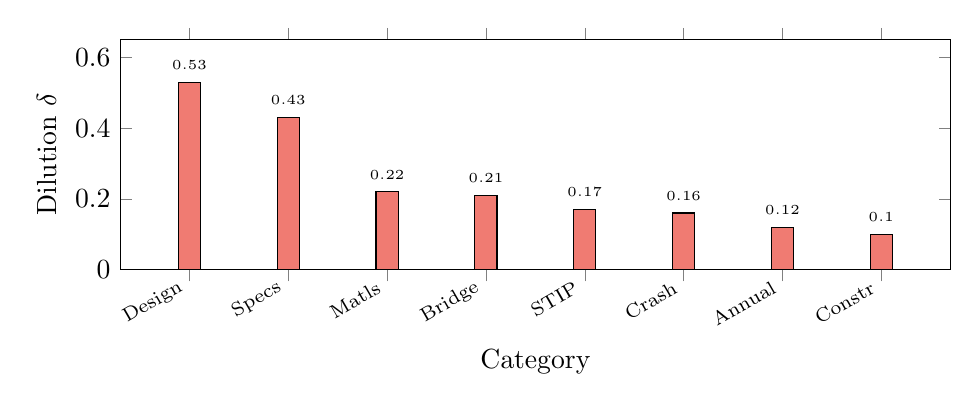
\begin{tikzpicture}
\begin{axis}[
    ybar,
    width=\columnwidth,
    height=4.5cm,
    bar width=8pt,
    xlabel={Category},
    ylabel={Dilution $\delta$},
    ymin=0, ymax=0.65,
    symbolic x coords={Design,Specs,Matls,Bridge,STIP,Crash,Annual,Constr},
    xtick=data,
    x tick label style={rotate=30, anchor=east, font=\scriptsize},
    nodes near coords,
    nodes near coords style={font=\tiny, above},
    every node near coord/.append style={yshift=1pt},
    enlarge x limits=0.1,
]
\addplot[fill=dilutionred!70] coordinates {
    (Design, 0.53)
    (Specs, 0.43)
    (Matls, 0.22)
    (Bridge, 0.21)
    (STIP, 0.17)
    (Crash, 0.16)
    (Annual, 0.12)
    (Constr, 0.10)
};
\end{axis}
\end{tikzpicture}
\caption{Dilution factor $\delta$ by category. Categories with fewer chunks suffer higher dilution, consistent with embedding space contamination from high-volume categories.}
\label{fig:dilution}
\end{figure}

\section{Routing Prompt}
\label{app:routing_prompt}

\begin{lstlisting}[basicstyle=\ttfamily\scriptsize]
You are a query router for WYDOT.
Classify into ONE category:
- STANDARD_SPECS: Construction specs,
  materials requirements, methods
- CONSTRUCTION_MANUAL: Field inspection,
  project administration
- MATERIALS_TESTING: Lab procedures,
  test methods, QC
- DESIGN_MANUAL: Road/bridge design,
  CADD standards
- TRAFFIC_CRASHES: Crash statistics,
  fatality data, trends
- STIP: Project funding, transportation
  improvement programs
- ANNUAL_REPORT: Department reports,
  accomplishments
- BRIDGE_PROGRAM: Bridge plans, ratings,
  load postings
- HIGHWAY_SAFETY: Safety programs, SHSP
- GENERAL: Cross-domain or unclear.

Format:
CATEGORY: <category>
YEAR: <year or NONE>
SERIES: <series or NONE>

Query: {query}
\end{lstlisting}

\section{Agent Scoped Filters}
\label{app:filters}

\begin{table}[H]
\centering
\footnotesize
\begin{tabular}{l l}
\toprule
\textbf{Agent} & \textbf{Filter (regex on document\_series)} \\
\midrule
specs & \texttt{(?i).*standard.spec.*} \\
construction & \texttt{(?i).*construction.manual.*} \\
materials & \texttt{(?i).*materials.*test.*} \\
design & \texttt{(?i).*design.manual.*} \\
safety & \texttt{(?i).*(crash|safety|fatal).*} \\
bridge & \texttt{(?i).*bridge.*(prog|plan).*} \\
planning & \texttt{(?i).*(stip|improv.prog).*} \\
admin & \texttt{(?i).*(annual.rep|strateg).*} \\
general & (no filter -- full corpus) \\
\bottomrule
\end{tabular}
\caption{Agent document\_series filters applied as Cypher WHERE clauses.}
\label{tab:agent_filters}
\end{table}

\section{Full Evaluation Results}
\label{app:full_results}

\begin{table*}[h]
\centering
\scriptsize
\begin{tabular}{p{4.5cm}lccccc}
\toprule
\textbf{Query (truncated)} & \textbf{Target} & \textbf{System} & \textbf{P@10} & \textbf{Correct} & \textbf{Faith.} & \textbf{Relev.} \\
\midrule
\multicolumn{7}{l}{\textit{Single-domain queries (113 total, representative sample):}} \\
Construction Limits definition & STD\_SPECS & \hybridname{} & 0.30 & \checkmark & 0.20 & 1.00 \\
 & & \systemname{} & 0.00 & \checkmark & 0.00 & 1.00 \\
Temporary stream crossing 404 permit & STD\_SPECS & \hybridname{} & 0.50 & \checkmark & 1.00 & 1.00 \\
 & & \systemname{} & 1.00 & \checkmark & 0.50 & 1.00 \\
Safety at active crusher site & CONSTR & \hybridname{} & 1.00 & \checkmark & 0.90 & 1.00 \\
 & & \systemname{} & 1.00 & \checkmark & 0.50 & 1.00 \\
\midrule
\multicolumn{7}{l}{\textit{Cross-domain queries (31 total, representative sample):}} \\
Bridge design vs.\ construction & DESIGN+CONSTR & \systemname{} & 1.00 & \checkmark & 0.40 & 1.00 \\
Safety improvements in STIP & SAFETY+STIP & \systemname{} & 1.00 & \texttimes & 0.20 & 1.00 \\
\midrule
\multicolumn{7}{l}{\textit{Version comparison (27 total, representative sample):}} \\
Aggregate gradation 2010 vs 2021 & STD\_SPECS & \systemname{} & 1.00 & \checkmark & 0.50 & 1.00 \\
\bottomrule
\end{tabular}
\caption{Representative per-query results for \systemname{} and \hybridname{}. Full \numQueries{}-query results for all 5 systems available in supplementary materials.}
\label{tab:full_results}
\end{table*}

\section{Statistical Test Details}
\label{app:stats}

\begin{table}[H]
\centering
\footnotesize
\begin{tabular}{l c c c}
\toprule
\textbf{System vs.\ Mono.} & \textbf{$p$(P@10)} & \textbf{$p$(Faith.)} & \textbf{$p$(Corr.)} \\
\midrule
Mono+RRF      & 0.511 & 0.304 & 0.821 \\
LLM+Scoped    & \textbf{0.038} & 0.973 & 0.809 \\
\systemname{} & \textbf{0.017} & \textbf{$<$0.001} & 0.102 \\
\hybridname{} & 0.107 & 0.901 & 0.912 \\
\midrule
\hybridname{} vs.\ \systemname{} & 0.323 & \textbf{$<$0.001} & -- \\
\bottomrule
\end{tabular}
\caption{Permutation test $p$-values (10,000 permutations). Bold: $p < 0.05$.}
\label{tab:pvalues}
\end{table}

\section{System Prompts}
\label{app:prompts}
\begin{lstlisting}[basicstyle=\ttfamily\scriptsize]
You are the WYDOT Knowledge Graph Assistant.
Answer questions about Wyoming Department of
Transportation using a knowledge graph with
1,128 documents and 88,907 text chunks.

IMPORTANT: You must ALWAYS call at least one
search tool for EVERY query. Never refuse a
query without searching first.

For each user query:
1. DECIDE which tool(s) to call based on topic
2. CALL the appropriate tool(s) with a clear
   search query
3. READ the returned document chunks carefully
4. SYNTHESIZE a comprehensive answer with
   citations

CITATION RULES:
- Reference sources as [Source 1], [Source 2]
- Include document title, section, and year
- If information comes from multiple sources,
  cite all of them

MULTI-STEP REASONING:
- For comparison queries, call compare_versions
  or call the same tool with different years
- For cross-domain queries, call multiple tools
- You can make up to 5 tool calls per query

ANSWER FORMAT:
- Use markdown with headers, bullet points,
  and tables where appropriate
- Be thorough but concise
- Always ground answers in retrieved content
\end{lstlisting}

\end{document}
